% Options for packages loaded elsewhere
\PassOptionsToPackage{unicode}{hyperref}
\PassOptionsToPackage{hyphens}{url}
%
\documentclass[
  man]{apa6}
\usepackage{amsmath,amssymb}
\usepackage{lmodern}
\usepackage{iftex}
\ifPDFTeX
  \usepackage[T1]{fontenc}
  \usepackage[utf8]{inputenc}
  \usepackage{textcomp} % provide euro and other symbols
\else % if luatex or xetex
  \usepackage{unicode-math}
  \defaultfontfeatures{Scale=MatchLowercase}
  \defaultfontfeatures[\rmfamily]{Ligatures=TeX,Scale=1}
\fi
% Use upquote if available, for straight quotes in verbatim environments
\IfFileExists{upquote.sty}{\usepackage{upquote}}{}
\IfFileExists{microtype.sty}{% use microtype if available
  \usepackage[]{microtype}
  \UseMicrotypeSet[protrusion]{basicmath} % disable protrusion for tt fonts
}{}
\makeatletter
\@ifundefined{KOMAClassName}{% if non-KOMA class
  \IfFileExists{parskip.sty}{%
    \usepackage{parskip}
  }{% else
    \setlength{\parindent}{0pt}
    \setlength{\parskip}{6pt plus 2pt minus 1pt}}
}{% if KOMA class
  \KOMAoptions{parskip=half}}
\makeatother
\usepackage{xcolor}
\usepackage{graphicx}
\makeatletter
\def\maxwidth{\ifdim\Gin@nat@width>\linewidth\linewidth\else\Gin@nat@width\fi}
\def\maxheight{\ifdim\Gin@nat@height>\textheight\textheight\else\Gin@nat@height\fi}
\makeatother
% Scale images if necessary, so that they will not overflow the page
% margins by default, and it is still possible to overwrite the defaults
% using explicit options in \includegraphics[width, height, ...]{}
\setkeys{Gin}{width=\maxwidth,height=\maxheight,keepaspectratio}
% Set default figure placement to htbp
\makeatletter
\def\fps@figure{htbp}
\makeatother
\setlength{\emergencystretch}{3em} % prevent overfull lines
\providecommand{\tightlist}{%
  \setlength{\itemsep}{0pt}\setlength{\parskip}{0pt}}
\setcounter{secnumdepth}{-\maxdimen} % remove section numbering
% Make \paragraph and \subparagraph free-standing
\ifx\paragraph\undefined\else
  \let\oldparagraph\paragraph
  \renewcommand{\paragraph}[1]{\oldparagraph{#1}\mbox{}}
\fi
\ifx\subparagraph\undefined\else
  \let\oldsubparagraph\subparagraph
  \renewcommand{\subparagraph}[1]{\oldsubparagraph{#1}\mbox{}}
\fi
\newlength{\cslhangindent}
\setlength{\cslhangindent}{1.5em}
\newlength{\csllabelwidth}
\setlength{\csllabelwidth}{3em}
\newlength{\cslentryspacingunit} % times entry-spacing
\setlength{\cslentryspacingunit}{\parskip}
\newenvironment{CSLReferences}[2] % #1 hanging-ident, #2 entry spacing
 {% don't indent paragraphs
  \setlength{\parindent}{0pt}
  % turn on hanging indent if param 1 is 1
  \ifodd #1
  \let\oldpar\par
  \def\par{\hangindent=\cslhangindent\oldpar}
  \fi
  % set entry spacing
  \setlength{\parskip}{#2\cslentryspacingunit}
 }%
 {}
\usepackage{calc}
\newcommand{\CSLBlock}[1]{#1\hfill\break}
\newcommand{\CSLLeftMargin}[1]{\parbox[t]{\csllabelwidth}{#1}}
\newcommand{\CSLRightInline}[1]{\parbox[t]{\linewidth - \csllabelwidth}{#1}\break}
\newcommand{\CSLIndent}[1]{\hspace{\cslhangindent}#1}
\ifLuaTeX
\usepackage[bidi=basic]{babel}
\else
\usepackage[bidi=default]{babel}
\fi
\babelprovide[main,import]{english}
% get rid of language-specific shorthands (see #6817):
\let\LanguageShortHands\languageshorthands
\def\languageshorthands#1{}
% Manuscript styling
\usepackage{upgreek}
\captionsetup{font=singlespacing,justification=justified}

% Table formatting
\usepackage{longtable}
\usepackage{lscape}
% \usepackage[counterclockwise]{rotating}   % Landscape page setup for large tables
\usepackage{multirow}		% Table styling
\usepackage{tabularx}		% Control Column width
\usepackage[flushleft]{threeparttable}	% Allows for three part tables with a specified notes section
\usepackage{threeparttablex}            % Lets threeparttable work with longtable

% Create new environments so endfloat can handle them
% \newenvironment{ltable}
%   {\begin{landscape}\centering\begin{threeparttable}}
%   {\end{threeparttable}\end{landscape}}
\newenvironment{lltable}{\begin{landscape}\centering\begin{ThreePartTable}}{\end{ThreePartTable}\end{landscape}}

% Enables adjusting longtable caption width to table width
% Solution found at http://golatex.de/longtable-mit-caption-so-breit-wie-die-tabelle-t15767.html
\makeatletter
\newcommand\LastLTentrywidth{1em}
\newlength\longtablewidth
\setlength{\longtablewidth}{1in}
\newcommand{\getlongtablewidth}{\begingroup \ifcsname LT@\roman{LT@tables}\endcsname \global\longtablewidth=0pt \renewcommand{\LT@entry}[2]{\global\advance\longtablewidth by ##2\relax\gdef\LastLTentrywidth{##2}}\@nameuse{LT@\roman{LT@tables}} \fi \endgroup}

% \setlength{\parindent}{0.5in}
% \setlength{\parskip}{0pt plus 0pt minus 0pt}

% Overwrite redefinition of paragraph and subparagraph by the default LaTeX template
% See https://github.com/crsh/papaja/issues/292
\makeatletter
\renewcommand{\paragraph}{\@startsection{paragraph}{4}{\parindent}%
  {0\baselineskip \@plus 0.2ex \@minus 0.2ex}%
  {-1em}%
  {\normalfont\normalsize\bfseries\itshape\typesectitle}}

\renewcommand{\subparagraph}[1]{\@startsection{subparagraph}{5}{1em}%
  {0\baselineskip \@plus 0.2ex \@minus 0.2ex}%
  {-\z@\relax}%
  {\normalfont\normalsize\itshape\hspace{\parindent}{#1}\textit{\addperi}}{\relax}}
\makeatother

% \usepackage{etoolbox}
\makeatletter
\patchcmd{\HyOrg@maketitle}
  {\section{\normalfont\normalsize\abstractname}}
  {\section*{\normalfont\normalsize\abstractname}}
  {}{\typeout{Failed to patch abstract.}}
\patchcmd{\HyOrg@maketitle}
  {\section{\protect\normalfont{\@title}}}
  {\section*{\protect\normalfont{\@title}}}
  {}{\typeout{Failed to patch title.}}
\makeatother

\usepackage{xpatch}
\makeatletter
\xapptocmd\appendix
  {\xapptocmd\section
    {\addcontentsline{toc}{section}{\appendixname\ifoneappendix\else~\theappendix\fi\\: #1}}
    {}{\InnerPatchFailed}%
  }
{}{\PatchFailed}
\keywords{keywords\newline\indent Word count: X}
\DeclareDelayedFloatFlavor{ThreePartTable}{table}
\DeclareDelayedFloatFlavor{lltable}{table}
\DeclareDelayedFloatFlavor*{longtable}{table}
\makeatletter
\renewcommand{\efloat@iwrite}[1]{\immediate\expandafter\protected@write\csname efloat@post#1\endcsname{}}
\makeatother
\usepackage{lineno}

\linenumbers
\usepackage{csquotes}
\ifLuaTeX
  \usepackage{selnolig}  % disable illegal ligatures
\fi
\IfFileExists{bookmark.sty}{\usepackage{bookmark}}{\usepackage{hyperref}}
\IfFileExists{xurl.sty}{\usepackage{xurl}}{} % add URL line breaks if available
\urlstyle{same} % disable monospaced font for URLs
\hypersetup{
  pdftitle={O*Net Factor Analysis Project},
  pdfauthor={First Author1 \& Ernst-August Doelle1,2},
  pdflang={en-EN},
  pdfkeywords={keywords},
  hidelinks,
  pdfcreator={LaTeX via pandoc}}

\title{O*Net Factor Analysis Project}
\author{First Author\textsuperscript{1} \& Ernst-August Doelle\textsuperscript{1,2}}
\date{}


\shorttitle{SIOP\_FA}

\authornote{

Add complete departmental affiliations for each author here. Each new line herein must be indented, like this line.

Enter author note here.

The authors made the following contributions. First Author: Conceptualization, Writing - Original Draft Preparation, Writing - Review \& Editing; Ernst-August Doelle: Writing - Review \& Editing.

Correspondence concerning this article should be addressed to First Author, Postal address. E-mail: \href{mailto:my@email.com}{\nolinkurl{my@email.com}}

}

\affiliation{\vspace{0.5cm}\textsuperscript{1} Wilhelm-Wundt-University\\\textsuperscript{2} Konstanz Business School}

\begin{document}
\maketitle

Given the popularity of the Job Demands-Resources Theory {[}JD-R; Demerouti et al. (2001){]} in exploring questions related to everything from motivation to job design, we aim to explore the intersection between \emph{perceptions} of job demands and resources, and the broad set of job characteristics provided on O*Net. This project makes three contributions. We aim to first explore whether ratings of of O*Net item groupings align with the stated ``resources'' and ``demands'' presented in the job demands-resources theory. We then present evidence documenting whether O*Net job and task descriptors are similarly rated as resources, challenge- or hindrance demands, and lastly, whether such ratings differ across job categories/classifications.
Across two studies, a series of evaluations were made that used: 1) direct O*Net terminology (both descriptor and response option), and 2) JD-R influenced ratings of demand, challenge, or hindrance of different types of workers. Prior to a description of results, a brief overview of both the JD-R theory, the stress appraisal process, and O*Net is provided.

\hypertarget{the-job-demands-resources-theory}{%
\subsection{The Job demands-Resources Theory}\label{the-job-demands-resources-theory}}

The overarching context for this study is that of the job demands-resources theory, which is an expansion of the well-studied job demands-resources model (Demerouti et al., 2001). One of the major advantages of the job demands-resources theory is that it allows us to model both work environment and job characteristics via job resources and demands. \emph{Resources} include physical, psychological, social, or organizational aspects of the job that may help an employee achieve work goals, reduce job demands, or promote personal growth and development (Demerouti et al., 2001). In contrast, \emph{demands} include components of a job that require sustained effort, and as such, produce psychological or physiological strain (e.g., high work pressure is frequently cited as a common demand; Demerouti et al. (2001)).
Cognitively, the perception of an element of ones job as a resource or demand activates one of two distinct processes: either health impairment (resulting from demands) or motivation {[}resulting from resources; A. B. Bakker and Demerouti (2014){]}. Pertinent to the current study, demanding job characteristics are frequently associated with negative outcomes (e.g., A. Bakker et al., 2003), whereas job characteristics deemed resources have been associated with positive organizational outcomes like engagement and motivation (A. B. Bakker et al., 2007).

\hypertarget{objective-vs.-subjective-nature-of-demands-and-resources-the-role-of-appraisal}{%
\subsection{Objective vs.~Subjective Nature of Demands and Resources: The Role of Appraisal}\label{objective-vs.-subjective-nature-of-demands-and-resources-the-role-of-appraisal}}

Searle and Auton (2015) note that the majority of the research on workplace demands is based on apriori classifications of demands. However, the stress experience, or process, described early on by Lazarus and Folkman (1984) is grounded in the assumption that individual appraisals of stressors/demands vary. Their transactional theory of stress and coping states that people continuously appraise stimuli in their environments. An appraisal is the cognitive process whereby meaning is assigned to a stimulus. If a stimulus is appraised as a stressor (threat, challenge, potentially harmful), emotional distress leads to coping of some kind. This action to cope is also associated with another appraisal about the outcome itself and the process continues if the outcomes is not appraised as favorable (Lazarus \& Folkman, 1984). The stress appraisal process suggests that classifying a job characteristic or environmental condition as an objective demand or resource might be in error.

We next consider the (limited) empirical evidence on this topic. First, some relatively recent research suggests that job demands and resources may not be universally appraised or assigned as such. Starting with job demands, Webster et al. (2011), for example, studied workload, role ambiguity, and role conflict demands, and found that while each could be appraised primarily as a challenge or hindrance demand, they could also simultaneously be perceived as being both a challenge and hindrance to different degrees. While their study did include resources, it nonetheless points to individual differences on how people perceive stressors at work. Although part of a much larger study on retirement, Sonnega et al. (2018) compared self-reported (subjective) ratings of degree of physical demand, stress, and need for intense concentration from the Health and Retirement Study with objective ratings from O*Net. Correlations physical demand (r = .52), stress (r = .10), and need for intense concentration (r = .14), again suggesting perhaps that our objective ratings of job demands (and resources) may be subject to a greater level of individual difference than assumed. Next considering resources, Schmitz et al. (2019) also captured subjective and objective resources in their study of retirement. Correlations of composite variables for the resources of autonomy (r = .12. p \textgreater{} .01), recognition of work (r = .07, p \textgreater{} .01), and decision freedom (r = .08, p \textgreater{} .01), while significant, certainly do not reflect high levels of overlap.

We do acknowledge as well, that demands and resources are not necessarily consistent across days, or seasons, for many employees. Downes et al. (2021) meta-analysis addresses this reality in depth, although it is beyond the scope of this project.

\hypertarget{onet-resource}{%
\subsection{O*Net Resource}\label{onet-resource}}

Originally, the Advisory Panel for the Dictionary of Occupational Titles recommended a system that would ``\ldots promote the effective education, training, counseling, and employment of the American workforce. It should accomplish its purpose by providing a database system that identifies, defines, classifies, and describes occupations in the economy in an accessible and flexible manner'' (Dictionary of Occupational Titles (US) and Service (1993), p.~6). The result was the now commonly used O*NET. The Occupational Information Network (O*NET; onetonline.org) contains a comprehensive description of occupations (Peterson et al., 2001). This widely accessed database houses hundreds of standardized and occupation-specific descriptors most occupations in the US and these descriptions are continually updated. In fact, there was a call to work with experienced I/O psychologists over the summer to update the content for the \href{https://www.onetonline.org/link/summary/19-3032.00}{Industrial and Organizational Psychologist listing on O*Net}. These data, and the tools provided for free on the website (e.g., Career Exploration Tools, ``My Next Move for Veterans'', ``My Next Move'', Toolkit for Business) are frequently used by counselors, students, human resources departments, and researchers to assist potential applicants discover the skills and training they need for the job of their choice. It is also useful to employers by providing them with information with which to craft job descriptions and help employees determine what skills are needed for promotion.

Of greatest interest here are statements taken from O*NET \href{https://www.O*NETonline.org/find/descriptor/result/4.A.1.b.3}{``activity'' and ``context'' classifications} (e.g., items related to information input, interacting with others, physical work conditions, structural job characteristics). One of the first and basic questions is whether or not the categorical examples of ``resources'' and ``demands'' described in the Job Demands-Resources Theory (Demerouti et al., 2001), for example, are generally deemed resources or demands as we objectively define them. The next logical question surrounds how ``universal'' such ratings are. For instance, it is quite possible, given the theoretical and empirical evidence presented above, that there is wide variability in individual appraisal of work activities and context such that some people may rate a given activity as a resource and others a hindrance. A second study extends the findings from Study 1 to a potentially key moderator - job categories/classifications, examining whether ratings of resources, challenge- and hindrance demands differ by job classification.

\hypertarget{methods}{%
\section{Methods}\label{methods}}

\hypertarget{participants}{%
\subsection{Participants}\label{participants}}

There were 568 respondents.

\hypertarget{participants-1}{%
\subsubsection{Participants}\label{participants-1}}

\begin{itemize}
\tightlist
\item
  568 respondents, 13.57\% had been in their referent job less than 6 months, 19.20\% between 6 months and a year, 49.12\% between one and five years, 13.27\% between 5 and 10 years, and 4.87\% more than 10 years.
\item
  Ages ranged from 18 to 65 with an average of 28.18 years old (SD = 7.53).
\item
  Gender: female (52.58\%) or male (46.83\%).
\item
  Job classifications: International Standard Classification of Occupations (ISCO) via the package \texttt{labourR} (\textbf{R-labourR?}), and further categorized into ``knowledge'' (n = 320) versus ``skilled'' (n = 214) occupations with knowledge workers being identified via ISCO classifications of: 1) professionals, and 2) managers.
\end{itemize}

The data for this study were collected through Prolific sample,18 or older and holding a full-time or part-time job. Participants were asked to think about their primary job while answering the survey, and upon completion each participant was compensated in the amount of six US dollars.

\hypertarget{materials}{%
\section{Materials}\label{materials}}

We used 98 statements taken directly from O\(^{*}\)Net's ``activity'' and ``context'' classifications. Each of the 98 descriptors has potentially unique response categories, but scaling was consistently 1 (low) to 5 (high). Subsequent to these self-evaluations, respondents were asked to rate elements in terms of 1) \ldots this aspect of your job is a resource that can be functional in achieving work goals, reduce job demands, or stimulate personal growth/development, 2) \ldots this aspect of your job is a challenge that can promote mastery, personal growth, or future gains, and 3) \ldots this aspect of your job is a hindrance that can inhibit personal growth, learning, and work goal attainment.

\hypertarget{procedure}{%
\subsection{Procedure}\label{procedure}}

We used PROCESS for R Version 4.1.1 (Hayes, 2022) to assess the extent to which the relationship between demands and stress are moderated by resources.

\hypertarget{results}{%
\section{Results}\label{results}}

\begin{verbatim}
## 
## ********************* PROCESS for R Version 4.1.1 ********************* 
##  
##            Written by Andrew F. Hayes, Ph.D.  www.afhayes.com              
##    Documentation available in Hayes (2022). www.guilford.com/p/hayes3   
##  
## *********************************************************************** 
##  
## PROCESS is now ready for use.
## Copyright 2022 by Andrew F. Hayes ALL RIGHTS RESERVED
## Workshop schedule at http://haskayne.ucalgary.ca/CCRAM
## 
\end{verbatim}

\begin{verbatim}
## 
## ********************* PROCESS for R Version 4.1.1 ********************* 
##  
##            Written by Andrew F. Hayes, Ph.D.  www.afhayes.com              
##    Documentation available in Hayes (2022). www.guilford.com/p/hayes3   
##  
## *********************************************************************** 
##                          
## Model : 1                
##     Y : stress           
##     X : overall.hindrance
##     W : overall.resource 
## 
## Sample size: 568
## 
## 
## *********************************************************************** 
## Outcome Variable: stress
## 
## Model Summary: 
##           R      R-sq       MSE         F       df1       df2         p
##      0.1311    0.0172    0.7790    3.2876    3.0000  564.0000    0.0205
## 
## Model: 
##                       coeff        se         t         p      LLCI      ULCI
## constant             1.2688    1.0055    1.2618    0.2075   -0.7063    3.2439
## overall.hindrance    0.8336    0.4031    2.0677    0.0391    0.0417    1.6254
## overall.resource     0.3319    0.2518    1.3181    0.1880   -0.1627    0.8264
## Int_1               -0.1918    0.1024   -1.8725    0.0616   -0.3929    0.0094
## 
## Product terms key:
## Int_1  :  overall.hindrance  x  overall.resource      
## 
## Test(s) of highest order unconditional interaction(s):
##       R2-chng         F       df1       df2         p
## X*W    0.0061    3.5064    1.0000  564.0000    0.0616
## ----------
## Focal predictor: overall.hindrance (X)
##       Moderator: overall.resource (W)
## 
## Conditional effects of the focal predictor at values of the moderator(s):
##   overall.resource    effect        se         t         p      LLCI      ULCI
##             3.2983    0.2010    0.0802    2.5065    0.0125    0.0435    0.3586
##             3.7402    0.1163    0.0534    2.1759    0.0300    0.0113    0.2213
##             4.2063    0.0269    0.0594    0.4535    0.6503   -0.0897    0.1435
## 
## Moderator value(s) defining Johnson-Neyman significance region(s):
##       Value   % below   % above
##      3.8196   55.6338   44.3662
## 
## Conditional effect of focal predictor at values of the moderator:
##   overall.resource    effect        se         t         p      LLCI      ULCI
##             1.0149    0.6389    0.3003    2.1276    0.0338    0.0491    1.2288
##             1.2078    0.6020    0.2809    2.1433    0.0325    0.0503    1.1536
##             1.4006    0.5650    0.2615    2.1608    0.0311    0.0514    1.0785
##             1.5935    0.5280    0.2421    2.1807    0.0296    0.0524    1.0035
##             1.7863    0.4910    0.2228    2.2034    0.0280    0.0533    0.9287
##             1.9791    0.4540    0.2037    2.2293    0.0262    0.0540    0.8540
##             2.1720    0.4170    0.1846    2.2592    0.0243    0.0545    0.7796
##             2.3648    0.3801    0.1657    2.2937    0.0222    0.0546    0.7055
##             2.5577    0.3431    0.1470    2.3336    0.0200    0.0543    0.6318
##             2.7505    0.3061    0.1287    2.3791    0.0177    0.0534    0.5588
##             2.9434    0.2691    0.1108    2.4292    0.0154    0.0515    0.4867
##             3.1362    0.2321    0.0937    2.4784    0.0135    0.0482    0.4161
##             3.3290    0.1951    0.0778    2.5085    0.0124    0.0423    0.3479
##             3.5219    0.1582    0.0641    2.4667    0.0139    0.0322    0.2841
##             3.7147    0.1212    0.0543    2.2306    0.0261    0.0145    0.2279
##             3.8196    0.1011    0.0515    1.9642    0.0500    0.0000    0.2021
##             3.9076    0.0842    0.0507    1.6605    0.0974   -0.0154    0.1838
##             4.1004    0.0472    0.0545    0.8662    0.3867   -0.0599    0.1543
##             4.2933    0.0102    0.0644    0.1589    0.8738   -0.1163    0.1368
##             4.4861   -0.0267    0.0782   -0.3421    0.7324   -0.1803    0.1268
##             4.6790   -0.0637    0.0941   -0.6773    0.4985   -0.2485    0.1211
##             4.8718   -0.1007    0.1112   -0.9054    0.3656   -0.3192    0.1178
## 
## Data for visualizing the conditional effect of the focal predictor:
##   overall.hindrance overall.resource    stress
##              1.6667           3.2983    2.6985
##              2.2894           3.2983    2.8237
##              3.2416           3.2983    3.0151
##              1.6667           3.7402    2.7039
##              2.2894           3.7402    2.7763
##              3.2416           3.7402    2.8871
##              1.6667           4.2063    2.7096
##              2.2894           4.2063    2.7264
##              3.2416           4.2063    2.7520
## 
## ******************** ANALYSIS NOTES AND ERRORS ************************ 
## 
## Level of confidence for all confidence intervals in output: 95
## 
## W values in conditional tables are the 16th, 50th, and 84th percentiles.
\end{verbatim}

\begin{figure}
\centering
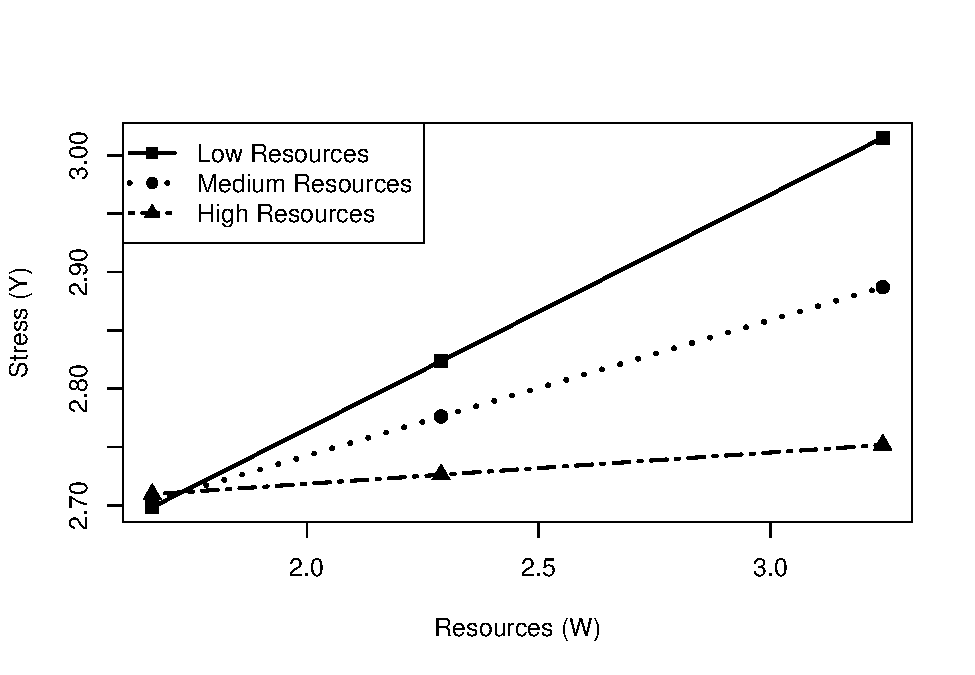
\includegraphics{SIOP_Onet_FA_files/figure-latex/analyses-1.pdf}
\caption{\label{fig:analyses}Interaction between hindrances and resources as predictors of stress}
\end{figure}

\hypertarget{discussion}{%
\section{Discussion}\label{discussion}}

\newpage

\hypertarget{references}{%
\section{References}\label{references}}

\begingroup
\setlength{\parindent}{-0.5in}
\setlength{\leftskip}{0.5in}

\hypertarget{refs}{}
\begin{CSLReferences}{1}{0}
\leavevmode\vadjust pre{\hypertarget{ref-bakker2014job}{}}%
Bakker, A. B., \& Demerouti, E. (2014). Job demands--resources theory. \emph{Wellbeing: A Complete Reference Guide}, 1--28.

\leavevmode\vadjust pre{\hypertarget{ref-bakker2007job}{}}%
Bakker, A. B., Hakanen, J. J., Demerouti, E., \& Xanthopoulou, D. (2007). Job resources boost work engagement, particularly when job demands are high. \emph{Journal of Educational Psychology}, \emph{99}(2), 274.

\leavevmode\vadjust pre{\hypertarget{ref-bakker2003dual}{}}%
Bakker, A., Demerouti, E., \& Schaufeli, W. (2003). Dual processes at work in a call centre: An application of the job demands--resources model. \emph{European Journal of Work and Organizational Psychology}, \emph{12}(4), 393--417.

\leavevmode\vadjust pre{\hypertarget{ref-demerouti2001job}{}}%
Demerouti, E., Bakker, A. B., Nachreiner, F., \& Schaufeli, W. B. (2001). The job demands-resources model of burnout. \emph{Journal of Applied Psychology}, \emph{86}(3), 499.

\leavevmode\vadjust pre{\hypertarget{ref-advisory1993new}{}}%
Dictionary of Occupational Titles (US), A. P. for the, \& Service, U. S. E. (1993). \emph{The new DOT: A database of occupational titles for the twenty-first century}. US Department of Labor, Employment; Training Administration, US~\ldots.

\leavevmode\vadjust pre{\hypertarget{ref-downes2021incorporating}{}}%
Downes, P. E., Reeves, C. J., McCormick, B. W., Boswell, W. R., \& Butts, M. M. (2021). Incorporating job demand variability into job demands theory: A meta-analysis. \emph{Journal of Management}, \emph{47}(6), 1630--1656.

\leavevmode\vadjust pre{\hypertarget{ref-hayes2022}{}}%
Hayes, A. F. (2022). \emph{Introduction to mediation, moderation, and conditional process analysis: A regression-based approach} (3rd ed.). The Guilford Press.

\leavevmode\vadjust pre{\hypertarget{ref-lazarus1984stress}{}}%
Lazarus, R. S., \& Folkman, S. (1984). \emph{Stress, appraisal, and coping}. Springer publishing company.

\leavevmode\vadjust pre{\hypertarget{ref-peterson2001understanding}{}}%
Peterson, N. G., Mumford, M. D., Borman, W. C., Jeanneret, P. R., Fleishman, E. A., Levin, K. Y., Campion, M. A., Mayfield, M. S., Morgeson, F. P., Pearlman, K., et al. (2001). Understanding work using the occupational information network (o* NET): Implications for practice and research. \emph{Personnel Psychology}, \emph{54}(2), 451--492.

\leavevmode\vadjust pre{\hypertarget{ref-schmitz_interpreting_2019}{}}%
Schmitz, L. L., McCluney, C. L., Sonnega, A., \& Hicken, M. T. (2019). Interpreting {Subjective} and {Objective} {Measures} of {Job} {Resources}: {The} {Importance} of {Sociodemographic} {Context}. \emph{International Journal of Environmental Research and Public Health}, \emph{16}(17), 3058. \url{https://doi.org/10.3390/ijerph16173058}

\leavevmode\vadjust pre{\hypertarget{ref-searle2015merits}{}}%
Searle, B. J., \& Auton, J. C. (2015). The merits of measuring challenge and hindrance appraisals. \emph{Anxiety, Stress, \& Coping}, \emph{28}(2), 121--143.

\leavevmode\vadjust pre{\hypertarget{ref-sonnega_comparison_2018}{}}%
Sonnega, A., Helppie-McFall, B., Hudomiet, P., Willis, R. J., \& Fisher, G. G. (2018). A {Comparison} of {Subjective} and {Objective} {Job} {Demands} and {Fit} {With} {Personal} {Resources} as {Predictors} of {Retirement} {Timing} in a {National} {U}.{S}. {Sample}. \emph{Work, Aging and Retirement}, \emph{4}(1), 37--51. \url{https://doi.org/10.1093/workar/wax016}

\leavevmode\vadjust pre{\hypertarget{ref-webster2011extending}{}}%
Webster, J. R., Beehr, T. A., \& Love, K. (2011). Extending the challenge-hindrance model of occupational stress: The role of appraisal. \emph{Journal of Vocational Behavior}, \emph{79}(2), 505--516.

\end{CSLReferences}

\endgroup


\end{document}
